\chapter{Sustav kontinuiranog razvoja na primjeru Web programa}
Za reviziju koda korišten je servis Github te je projekt nazvan \textit{diplomski-go}. Jenkins je
instaliran zajedno s osnovnim dodacima koji su potrebno za ovaj projekt - Pipeline, Git, Docker.
Nakon objave prve verzije programa, izrađen je Jenkins posao koji izgrađuje Docker sliku te
objavljuje na službeni Docker repositorij. Takvu sliku preuzima servis za menadžment te pokreće
Docker kontejner. Nakon što je kontejner spreman, Nginx počinje preusmjerivati zahtjeve na njega.

\section{Aplikacija za izračun fibonaccijevog broja}
Za testiranje kontinuiranog razvoja izrađena je web programa za izračun fibonaccijevog broja u Go
programskom jeziku. Fibonaccijev broj definiran je rekurzijskom relacijom:

\begin{equation*}
    f(n) = \begin{cases}
               0               & n = 0\\
               1               & n = 1\\
               f(n-1) + f(n-2) & n > 1
           \end{cases}
\end{equation*}

U prvoj iteraciji programa koristi se naivno, rekurzivno rješenje vremenske i memorijske
kompleksnosti $O(2^N)$. Prilikom primitka HTTP zahtjeva, programa pokreće računanje fibonaccijevog
broja tako da zbroji rješenja prijašnje dvije iteracije fibonaccijevog broja. Na primjer, ako je
zatražen broj pet, funkcija vraća zbroj dvije fibonacci funkcije, jedna s parametrom četiri, a druge
s tri. Implementacija je prikazana kodom~\ref{03fibv1} te slikom~\ref{fig:03fibv1png}

\begin{figure}[h]
    \centering
    
\includegraphics[width=0.3\textwidth]{img/03/fibonacci_html.png}
    \caption{Izgled fibonacci web aplikacije}%
    \label{fig:03fibv1png}
\end{figure}

\lstset{caption={Fibonacci v1}, label=03fibv1}
\begin{lstlisting}[float=h]
func fibonacci(n uint64) uint64 {
	if n == 0 {
		return 0
	} else if n == 1 {
		return 1
	} else {
		return fibonacci(n-1) + fibonacci(n-2)
	}
}
\end{lstlisting}

Kako bi se provjerila ispravnost koda, napisani su jednostavni testovi jedinice, prikazano
kodom~\ref{03fibunit} te \textit{end-to-end} testovi prikazani kodom~\ref{03fibe2e}.

\lstset{caption={Testiranje jedinice}, label=03fibunit}
\begin{lstlisting}[float=h]
func TestFibonacci(t *testing.T) {
	assert.Equal(t, uint64(5), fibonacci(5))
	assert.Equal(t, uint64(8), fibonacci(6))
	assert.Equal(t, uint64(89), fibonacci(11))
}
\end{lstlisting}

\lstset{caption={\textit{End-to-end} testiranje}, label=03fibe2e}
\begin{lstlisting}[language=php,float=h]
describe('Fibonacci test', function() {
    it("Ispravna forma", function() {
        cy.visit('/');

        cy.get('#number').type('11');
        cy.get('form').contains('Racunaj').click();
        cy.contains('89');
    });

    it("Neispravna forma", function() {
        cy.visit('/');

        cy.get('#number').type("-1");
        cy.get('form').contains('Racunaj').click();
        cy.contains('Parametar n mora biti prirodni broj.');
    });
})
\end{lstlisting}

U glavnoj funkciji koja se poziva prilikom pokretanje programa, \textit{main}, pokrenut je HTTP
servis koji je zadužen za posluživanje HTTP zahtjeva. Pokretanje HTTP servisa dan je
kodom~\ref{03fibhttp}.

\lstset{caption={HTTP servis}, label=03fibhttp}
\begin{lstlisting}[float=h]
func fibonacciHandler(w http.ResponseWriter, r *http.Request) {
	n, err := strconv.ParseUint(r.URL.Query().Get("n"), 10, 64)
	if err != nil {
		w.WriteHeader(http.StatusBadRequest)
		w.Write([]byte("Parametar n mora biti prirodni broj."))
		return
	}
	w.WriteHeader(http.StatusOK)
	w.Write([]byte(strconv.FormatUint(fibonacci(n), 10)))
}

func healthHandler(w http.ResponseWriter, r *http.Request) {
	w.WriteHeader(http.StatusOK)
	w.Write([]byte("OK"))
}

func homePageHandler(w http.ResponseWriter, r *http.Request) {
	http.ServeFile(w, r, "./static/index.html")
}

func main() {
	http.HandleFunc("/", homePageHandler)
	http.HandleFunc("/api/fibonacci", fibonacciHandler)
	http.HandleFunc("/health", healthHandler)

	log.Fatal(http.ListenAndServe(":8888", nil))
}

\end{lstlisting}

\section{Jenkins posao za izgradnju i objavu Docker slike}
Za Jenkins posao koji izrađuje Docker sliku i objavljuje u Docker repositorij odabrana je je Jenkins
linija. Jenkins linija je isprogramirana i spremljena u datoteci~\textit{Jenkinsfile} unutar
fibonacci projekta. Jenkins linija se sastoji od šest faza: dohvaćanje koda preko Git projekta,
pokretanje testova jedinica, izgradnja Docker slike, pokretanje \textit{end-to-end} testova te
objava Docker slike u javni Docker repositorij. Na slici~\ref{fig:03jenkins_pipeline} prikazana je
Jenkins linija.

\begin{figure}[h]
    \centering
    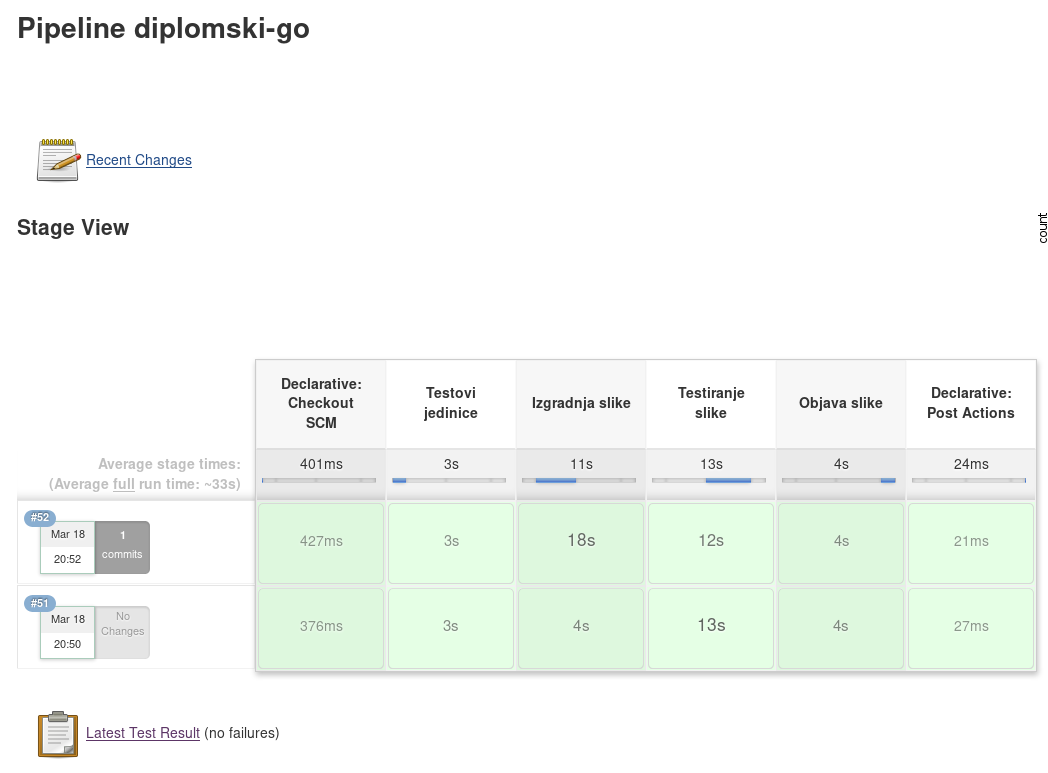
\includegraphics[width=0.8\textwidth]{img/03/jenkins_pipeline.png}
    \caption{Jenkins linija za izgradnju i objavu slike}%
    \label{fig:03jenkins_pipeline}
\end{figure}

Jenkins linija podešena je da periodički provjerava Git projekt, točnije svake minute. Ukoliko je
došlo do promjene u Git projektu, pokreće Jenkins liniju.

U prvoj fazi Jenkins kopira Git projekt koji se poslužuje preko Github servisa. Git projekt javno je
dostupan tako da nije potrebno podesiti autorizaciju. Nakon što je Git projekt kopiran, Jenkins
uspoređuje razliku između prijašnje i trenutnačne verzije te ih prikazuje korisniku.

U drugoj fazi pokreće se testovi jedinice unutar Docker kontejnera. Fibonacci aplikacija sastoji se
od jednog testa jedinice koji ispituje 3 ulaza. Ukoliko dođe do greške, Jenkins linija se prekida.
Pomoću ~\textit{junit} skripte, Jenkins objavljuje rezultate testova, kao i vrijeme izvođenja.

U trećoj fazi aplikacija se kompajlira i objavljuje sprema unutar Docker slike. Treća i druga faza
dijele istu baznu Docker sliku. Stoga, inženjer može biti siguran da su sve biblioteke dostupne
ukoliko su pokrivene testovima jedinice. Docker slika se označuje s trenutnom verzijom izgradnje
(\textit{engl. build number}) te se objavljuje na Docker repositorij. Kako bi se slika mogla
objaviti, potrebno je podesiti Docker autorizaciju unutar Jenkins sustava.

U četvrtoj fazi pokreće se \textit{end-to-end} testiranje pomoću Cypress alata. Jenkins pokreće
Docker kontejner koji pokreće zadnju verziju aplikacije izgrađenu u prethodnom koraku. Zatim, u
drugom Docker kontejernu pokreće Cypress alat. Cypress zatim pokreće testove koji komuniciraju sa
novom verzijom aplikacije. Rezultati se također objavljuju pomoću \textit{junit}.

U petoj fazi, Docker slika se označuje sa specijalnom oznakom \textit{latest}. Ta oznaka označuje
da je Docker slika spremna za uporabu od strane klijenata. Tu sliku dohvatit će servis za
menadžment.

U zadnjoj fazi, koja se bezuvjetno izvršava, prikupljaju se rezultati testova jedinica i
\textit{end-to-end} testiranja. Rezultati su vidljivi korisniku preko Jenkins web sučelje.

\section{Servis za menadžment}
Servis za menadžment je servis zadužen za preuzimanje zadnje Docker slike objavljene na
Docker repositoriju. Prilikom pokretanja servisa, korisnik mora podesiti konfiguracijku datoteku.
Konfiguracijska datoteka je datoteka u \textit{JSON} formatu koja sadrži informacije o Docker slici,
lokaciji Nginx PID datoteci, lokaciji Nginx datotečnoj konfiguracije te vrijeme čekanja prilikom
rotiranja verzije aplikacije. Primjer konfiguracije prikazan je kodom~\ref{03jsonconfig}.

\lstset{caption={JSON konfiguracija}, label=03jsonconfig}
\begin{lstlisting}[float=h]
{
    "dockerImage": "sokac/fibonacci",
    "nginxPIDfile": "/run/nginx.pid",
    "nginxConfiguration": "/tmp/nginx.conf",
    "versionOverlapDuration": 30
}

\end{lstlisting}

Informacija o nazivu Docker slike spremljena je pod ključem \textit{dockerImage}. Servis
zahtjeva da zadnja inačica slike ima oznaku \textit{latest}, a što je ujedno i Docker standard.

Nginx PID datoteka, spremljena pod ključem \textit{nginxPIDfile} sadrži indentitet Nginx procesa.
Pomoću tog indentiteta moguće je poslati zahtjev Nginx procesu da ponovno učita konfiguracije
datoteke bez prekida posluživanja korisnika.

Nginx datotečna konfiguracija sprema postavke potrebne da Nginx može prosljediti informacije
aplikaciji, to jest Docker kontejneru. Vrijednost je spremljena pod ključem
\textit{nginxConfiguration}. Primjer generirane konfiguracije prikazan je
kodom~\ref{03nginxconfig}.

\lstset{caption={Nginx konfiguracija}, label=03nginxconfig}
\begin{lstlisting}[float=h]
# Managed by Manager
upstream manager_backend {
    server 127.0.0.1:45105;
}
\end{lstlisting}

Nakon što servis pokrene Docker kontejner s novom aplikacijom, čekat će zadani broj sekundi prije
nego ugasi i obriše kontejner sa starom verijom aplikacije. Takvo vrijeme zadano je ključem
\textit{versionOverlapDuration}.

Ukoliko je konfiguracijska datoteka ispravna, servis počinje periodički provjeravati izmjene na
udaljenom repositoriju. Ukoliko je došlo do promjene slike s oznakom \textit{latest}, servis pokreće
novi Docker kontejner koji prihvaća zahtjeve na nekorištenom \textit{TCP portu}. Zatim zapisuje novu
Nginx konfiguraciju na tvrdi disk te šalje \textit{SIGHUP Unix} signal Nginx procesu. Takav signal
služi za učitanje promjena konfiguracije. Nakon korisničko definiranog vremena, stari Docker
kontejner se gasi te automatski briše. Dijagram toka prikazan je
slikom~\ref{fig:03servismanagement}.

\begin{figure}[h]
    \centering
    \begin{tikzpicture}[
        scale=1.0,
        node distance=1cm,
        text width=3.5cm,
        text centered,
        block/.style={
            rectangle,
            draw,
            text width=10em,
            text centered,
            rounded corners,
        },
        process/.style={
            rectangle,
            draw,
            text width=10em,
            text centered,
        },
        decision/.style={
            diamond,
            draw,
            text width=4em,
            text badly centered,
            inner sep=0pt,
        },
        arrow/.style={
            thick,->,>=stealth
        },
    ]
        \node [block] (start) {POČETAK};

        \node [process, below=of start] (checkversion) {Provjeri zadnju verziju slike};

        \node [left=of checkversion] (e2) {};

        \node [decision, below=of checkversion] (newversion) {Nova verzija?};

        \node [process, below=of newversion] (launch) {Pokreni najnoviju verziju u kontejneru};
        \node [process, below=of launch] (save) {Spremni novu Nginx konfiguraciju};
        \node [process, below=of save] (reload) {Učitaj Nginx promjene};
        \node [process, below=of reload] (shutdown) {Ugasi stari kontejner};

        \draw [arrow] (start) -- (checkversion);
        \draw [arrow] (checkversion) -- (newversion);
        \draw [arrow] (newversion) -- node[anchor=south] {NE} ++(-3cm,0cm) |- (checkversion);

        \draw [arrow] (newversion) -- node[xshift=-5mm] {DA} (launch);
        \draw [arrow] (launch) -- (save);
        \draw [arrow] (save) -- (reload);
        \draw [arrow] (reload) -- (shutdown);
        \draw [arrow] (shutdown) -- ++(+4.5cm,0cm) |- (checkversion);
    \end{tikzpicture}
    \caption{Dijagram toka servisa za menadžment}%
    \label{fig:03servismanagement}
\end{figure}

Generirana Nginx konfiguracija sadrži samo informacije o Docker kontejeru te kao takva nije potpuna.
Glavna Nginx konfiguracija priključuje takvu konfiguraciju glavnom pomoću direktive
\textit{include}. Primjer glavne Nginx konfiguracije prikazan je kodom~\ref{03nginxconfig2}.

\lstset{caption={Nginx konfiguracija}, label=03nginxconfig2}
\begin{lstlisting}[float=h]
worker_processes 1; # broj radnika

events {
    worker_connections  1024; # broj veza po radniku
}

http {
    include /tmp/nginx.conf; # Lokacija generirane Nginx konfiguracije

    keepalive_timeout  60; # Vrijeme koliko dugo ce veza biti otvorena

    server {
        listen       80; # Port slusanja
        server_name  localhost; # Domena

        location / {
            proxy_pass http://manager_backend; # Prosljedi zahtjev
        }
    }
}
\end{lstlisting}
